% This is a Basic Assignment Paper but with like Code and stuff allowed in it, there is also url, hyperlinks from contents included. 

\documentclass[11pt]{article}

% Preamble

\usepackage[margin=1in]{geometry}
\usepackage{amsfonts, amsmath, amssymb}
\usepackage{fancyhdr, float, graphicx}
\usepackage[utf8]{inputenc} % Required for inputting international characters
\usepackage[T1]{fontenc} % Output font encoding for international characters
\usepackage{fouriernc} % Use the New Century Schoolbook font
\usepackage[nottoc, notlot, notlof]{tocbibind}
\usepackage{listings}
\usepackage{xcolor}
\usepackage{blindtext}
\usepackage{hyperref}
\hypersetup{
    colorlinks=true,
    linkcolor=black,
    filecolor=magenta,      
    urlcolor=cyan,
    pdfpagemode=FullScreen,
    }

\definecolor{codegreen}{rgb}{0,0.6,0}
\definecolor{codegray}{rgb}{0.5,0.5,0.5}
\definecolor{codepurple}{rgb}{0.58,0,0.82}
\definecolor{backcolour}{rgb}{0.95,0.95,0.92}

\lstdefinestyle{mystyle}{
    backgroundcolor=\color{backcolour},   
    commentstyle=\color{codegreen},
    keywordstyle=\color{magenta},
    numberstyle=\tiny\color{codegray},
    stringstyle=\color{codepurple},
    basicstyle=\ttfamily\footnotesize,
    breakatwhitespace=false,         
    breaklines=true,                 
    captionpos=b,                    
    keepspaces=true,                 
    numbers=left,                    
    numbersep=5pt,                  
    showspaces=false,                
    showstringspaces=false,
    showtabs=false,                  
    tabsize=2
}

\lstset{style=mystyle}

% Header and Footer
\pagestyle{fancy}
\fancyhead{}
\fancyfoot{}
\fancyhead[L]{\textit{\Large{SET Assignment 7 - Component Diagrams}}}
%\fancyhead[R]{\textit{something}}
\fancyfoot[C]{\thepage}
\renewcommand{\footrulewidth}{1pt}



% Other Doc Editing
% \parindent 0ex
%\renewcommand{\baselinestretch}{1.5}

\begin{document}

\begin{titlepage}
	\centering

	%---------------------------NAMES-------------------------------

	\huge\textsc{
		MIT World Peace University
	}\\

	\vspace{0.75\baselineskip} % space after Uni Name

	\LARGE{
		Software Engineering and Testing\\
		Second Year B. Tech, Semester 4
	}

	\vfill % space after Sub Name

	%--------------------------TITLE-------------------------------

	\rule{\textwidth}{1.6pt}\vspace*{-\baselineskip}\vspace*{2pt}
	\rule{\textwidth}{0.6pt}
	\vspace{0.75\baselineskip} % Whitespace above the title



	\huge{\textsc{
			Component Diagrams and Deployment Diagrams
		}} \\



	\vspace{0.5\baselineskip} % Whitespace below the title
	\rule{\textwidth}{0.6pt}\vspace*{-\baselineskip}\vspace*{2.8pt}
	\rule{\textwidth}{1.6pt}

	\vspace{1\baselineskip} % Whitespace after the title block

	%--------------------------SUBTITLE --------------------------	

	\LARGE\textsc{
		\centering
		Assignment No. 7
	} % Subtitle or further description
	\vfill

	%--------------------------AUTHOR-------------------------------

	Prepared By
	\vspace{0.5\baselineskip} % Whitespace before the editors

	\Large{
		Krishnaraj Thadesar \\
		Cyber Security and Forensics\\
		Batch A1, PA 20
	}


	\vspace{0.5\baselineskip} % Whitespace below the editor list
	\today

\end{titlepage}


\tableofcontents
\thispagestyle{empty}
\clearpage

\setcounter{page}{1}

\section{Aim}
Object Oriented Analysis and design using UML diagrams: Component diagram, deployment diagram using Open Source Tool.

\section{Objectives}

\begin{enumerate}
	\item To learn the relationships and notions of Component diagram.
	\item To learn the relationships and notions of Deployment diagram.
\end{enumerate}

\section{Problem Statement}

\textbf{Draw Component Diagram and Deployment Diagram for The Following Problem:} \\

\textit{The Purpose of an Attandence Assistant App is to help reduce the time taken for recording the attendance of a classroom in a school or college. The app will be able to record the attendance of a class in a matter of a few Seconds with minimum Energy Expended. It will record data on cloud, and be accessible to all the Teachers.}\\

The tasks we have to do are:
\begin{enumerate}
	\item You will have to identify the main entities (objects) for this system.
	\item You will have to find out the relationships between these objects.
	\item You will have to find the necessary attributes and functions that need to be associated
	      with each object to implement the functionality mentioned above.
	\item You will make a final comprehensive diagram show and all objects and their relations
	      along with their attributes and functions.
\end{enumerate}

\section{Theory}

\subsection{Component Diagram}

\subsubsection{What is a Component Diagram}

\begin{quotation}
	A component diagram is a type of UML diagram that shows the physical components of a system and how they are interconnected. It is used to visualize, specify, and document the architecture and structure of a software system.
\end{quotation}

\subsubsection{What is the use of a Component Diagram}

\begin{enumerate}
	\item \textit{Identifying system components}: Component diagrams can be used to identify the various components of a system, including hardware, software, and other physical elements.
	\item \textit{Visualizing system architecture}: Component diagrams provide a visual representation of the system architecture, showing the relationships and dependencies between different components.
	\item \textit{Designing software systems}: Component diagrams can be used in software design to map out the different components of a system and their interactions.
	\item \textit{Testing and debugging}: Component diagrams can be used in testing and debugging to identify potential problems or bottlenecks in the system architecture.
	\item \textit{Communication}: Component diagrams are a useful tool for communicating system architecture and design to stakeholders and team members.
\end{enumerate}

\subsubsection{Elements of a Component Diagram}

\begin{enumerate}
	\item \textit{Component}: A component is a physical element or module of the system, such as a software module, hardware component, or database.
	\item \textit{Interface}: An interface defines the way in which a component communicates with other components in the system.
	\item \textit{Connector}: A connector shows the relationships and dependencies between different components and interfaces.
	\item \textit{Port}: A port is a specific point of connection between a component and an interface.
	\item \textit{Dependency}: A dependency shows the relationship between two components, indicating that one component depends on another for its operation
\end{enumerate}

\begin{figure}[H]
	\centering
	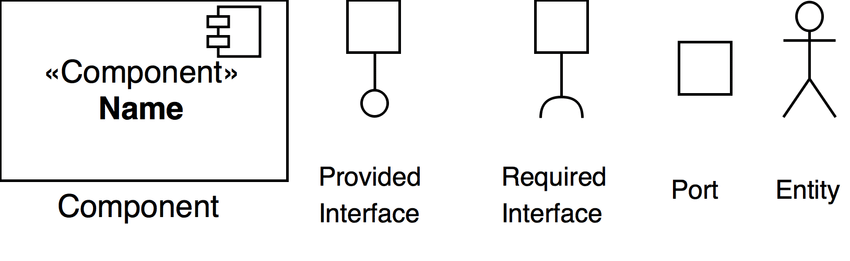
\includegraphics[width=.7\textwidth]{UML-component-diagram-notation-elements.png}
	\caption{Elements of a Component Diagram}
\end{figure}

% \clearpage 

\subsection{Deployment Diagram}

\subsubsection{What is a Deployment Diagram}
\begin{quotation}
	A deployment diagram is a type of UML diagram that shows the physical deployment of software components on hardware nodes. It depicts the architecture of a system as it is deployed to different hardware configurations, such as servers, workstations, or mobile devices.
\end{quotation}
\subsubsection{What is the use of a Deployment Diagram}

The main use of a deployment diagram is to model and visualize the physical deployment of software components within a system. Some specific uses of deployment diagrams include:

\begin{enumerate}
	\item \textit{Understanding system architecture}: Deployment diagrams provide a high-level view of the system architecture, showing how software components are deployed on hardware nodes.
	\item \textit{Designing and planning deployment}: Deployment diagrams can be used to plan the deployment of a system, helping to identify potential issues and dependencies between different components.
	\item \textit{Communication}: Deployment diagrams are a useful tool for communicating system architecture and deployment plans to stakeholders and team members.
	\item \textit{Testing and debugging}: Deployment diagrams can be used in testing and debugging to identify potential issues or bottlenecks in the deployment architecture.
	\item \textit{Scaling and optimization}: Deployment diagrams can be used to identify opportunities for scaling and optimizing the system architecture for improved performance and efficiency.

\end{enumerate}

\subsubsection{Elements of a Deployment Diagram}

\begin{enumerate}
	\item \textit{Node}: A node represents a physical device or server, such as a computer, printer, or mobile device.
	\item \textit{Component}: A component represents a software module or application that is deployed on a hardware node.
	\item \textit{Artifact}: An artifact is a physical element, such as a file or database, that is used by a software component.
	\item \textit{Deployment relationship}: A deployment relationship shows how components are deployed on nodes, including the mapping of artifacts to nodes.
	\item \textit{Communication path}: A communication path shows how nodes communicate with each other, including network connections, protocols, and other communication channels.
\end{enumerate}

\begin{figure}[H]
	\centering
	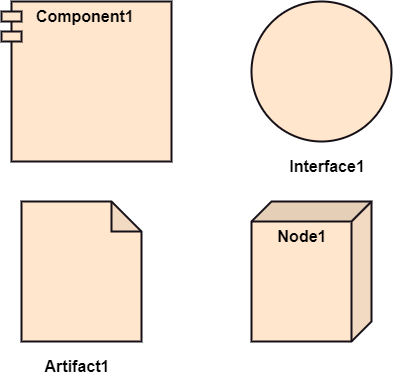
\includegraphics[width=.45\textwidth]{uml-deployment-diagram.png}
	\caption{Elements of a Deployment Diagram}
\end{figure}

\clearpage

\section{Diagrams}

\subsection{Component Diagram}

% \begin{figure}[H]
% \centering
% 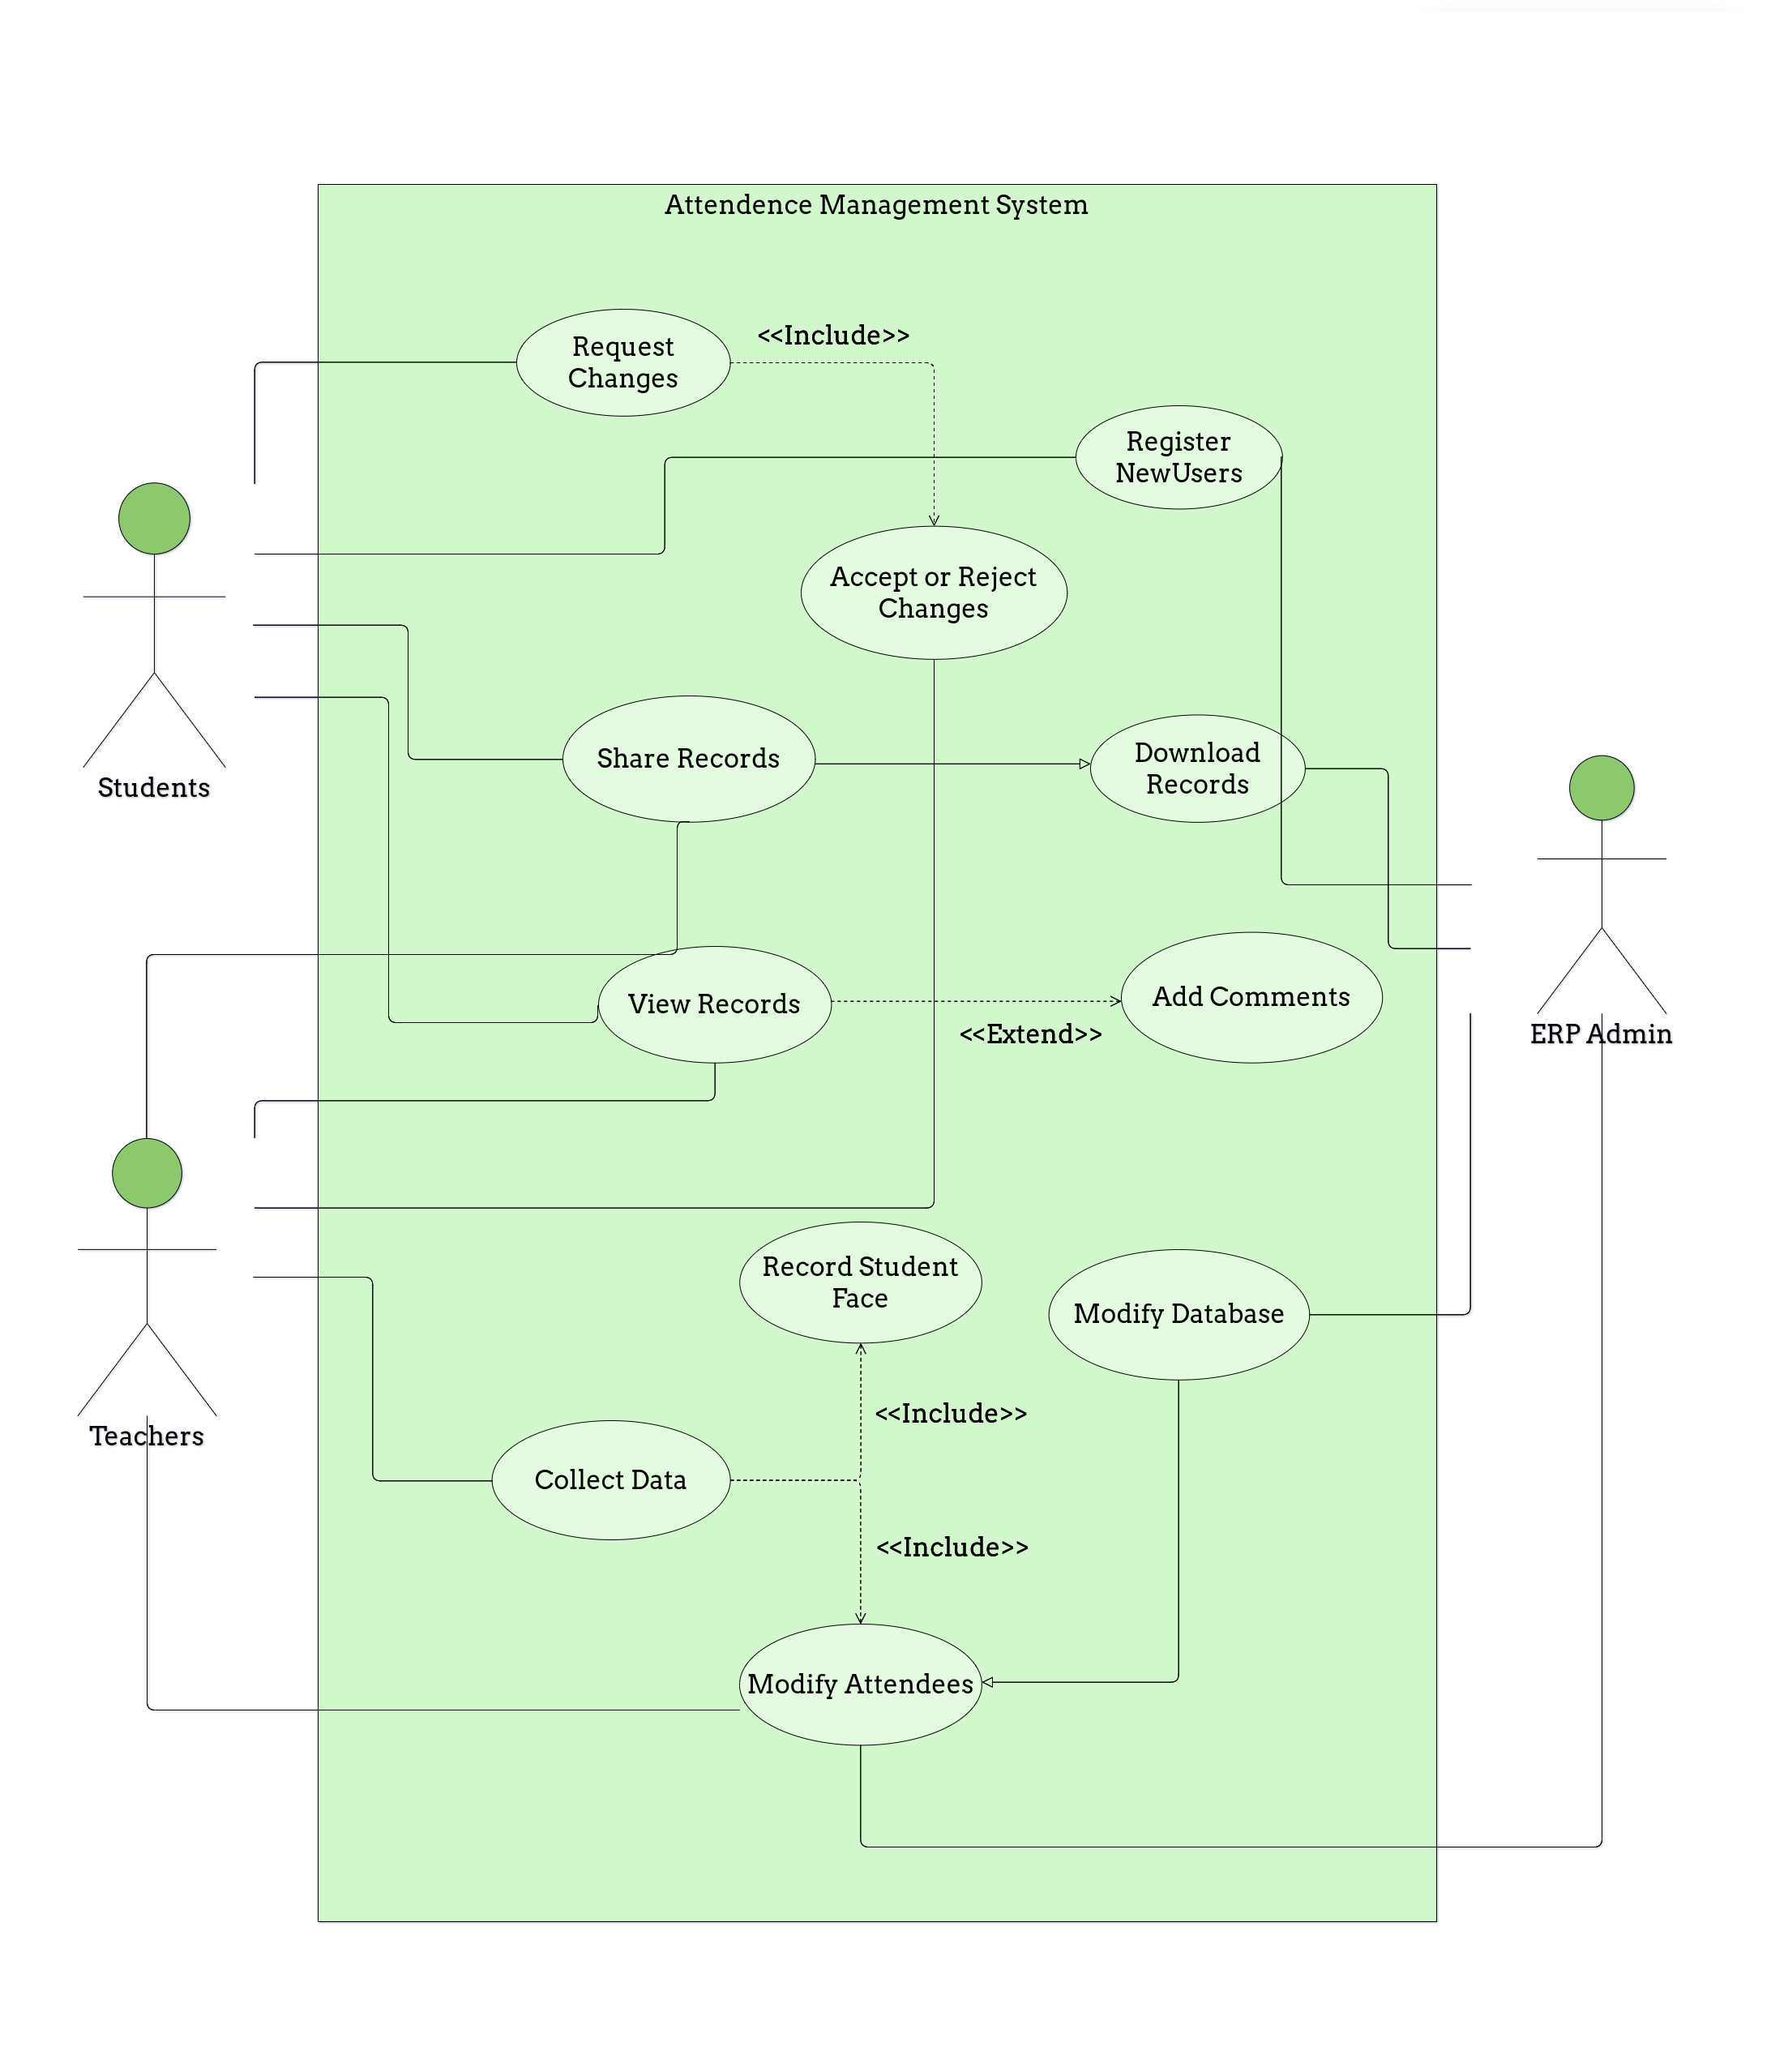
\includegraphics[scale=0.20]{use_case.png}
% \caption{Use Case Diagram}
% \end{figure}

\subsection{Deployment Diagram}

% \begin{figure}[H]
% 	\centering
% 	\includegraphics[scale=0.20]{class.png}
% 	\caption{Class Diagram}
% \end{figure}

\section{Platform}
\textbf{Operating System}: Arch Linux x86-64 \\
\textbf{IDEs or Text Editors Used}: Visual Studio Code\\
\textbf{External Programs for Diagrams} : Draw.io\\


\section{Conclusion}
Thus, we learnt about Component diagrams and Deployment diagrams. We also learnt about the different types of diagrams and their uses in detail.
\clearpage

\section{FAQ}
\begin{enumerate}
	\item \textbf{The term component is sometimes a difficult one to define. First provide a generic definition, and then provide more explicit definitions for object-oriented and traditional software. Finally, pick three programming languages with which you are familiar and illustrate how each defines a component.}\\
	
	\textit{A component is a modular, reusable, and independent part of a system that encapsulates a set of related functionality. It can be a physical or logical entity that can be easily integrated into other systems or applications.}\\

	In object-oriented software, a component is typically a class or group of classes that provide a specific set of functionalities. It is designed to be easily integrated into other object-oriented systems and can be easily extended or modified.\\
	
	In traditional software, a component is typically a set of functions or procedures that provide a specific set of functionalities. It is designed to be easily integrated into other traditional systems and can be easily modified or replaced.
	
	Three programming languages that define a component are:
	
	\begin{itemize}
		\item Java: In Java, a component is typically defined as a reusable software module that can be easily integrated into other Java applications. It is typically implemented as a Java class or set of classes that encapsulate a specific set of functionalities.
		
		\item Python: In Python, a component is typically defined as a module or package that provides a specific set of functionalities. It is designed to be easily integrated into other Python applications and can be easily extended or modified.
		
		\item C++: A component in C++ can be implemented as a class or set of classes that provide a specific set of functionalities, which can be easily integrated into other C++ applications. Additionally, C++ provides features like templates, namespaces, and libraries, which can be used to define and package reusable components for different purposes.
	\end{itemize}
	
	\item \textbf{What is a WebApp component?}\\

	A WebApp component is a modular and reusable part of a web application that encapsulates a specific set of functionalities. It can be a physical or logical entity that can be easily integrated into other web applications or systems. WebApp components typically include web pages, scripts, databases, and other resources that provide a specific set of functionalities within a web application.

	\item \textbf{Draw the deployment diagram for the university information system.}\\

	\item \textbf{State the importance of deployment diagram.}\\
	      The importance of a deployment diagram includes:
	      \begin{itemize}
		      \item Providing a high-level view of the physical deployment of software components within a system.
		      \item Helping to identify potential issues and dependencies between different components.
		      \item Aiding in system design, planning, and communication.
		      \item Identifying opportunities for scaling and optimizing the system architecture.
		      \item Assisting in testing and debugging to identify potential issues or bottlenecks in the deployment architecture.
	      \end{itemize}

\end{enumerate}
\end{document}